\documentclass[12pt]{article}
\usepackage{fullpage}
\usepackage[sc]{mathpazo} % Use the Palatino font
\usepackage[T1]{fontenc} % Use 8-bit encoding that has 256 glyphs
\linespread{1.75} % Line spacing - Palatino needs more space between lines

\usepackage{abstract}
\renewcommand{\abstractnamefont}{\normalfont\bfseries} % Set the "Abstract" text to bold
\renewcommand{\abstracttextfont}{\normalfont\small\itshape} % Set the abstract itself to small italic text


\usepackage{titlesec} % Allows customization of titles
\renewcommand\thesection{\Roman{section}} % Roman numerals for the sections
\renewcommand\thesubsection{\arabic{subsection}} % Roman numerals for subsections
\titleformat{\section}[block]{\large\scshape\centering}{\thesection.}{1em}{} % Change the look of the section titles
\titleformat{\subsection}[block]{\large}{\thesubsection.}{1em}{} % Change the look of the section titles

\usepackage{graphicx}
\graphicspath{ {images/} }


\title{\vspace{-15mm}\fontsize{24pt}{10pt}\selectfont\textbf{SVHN Classification}} % Article title
\author{
	\large
	\textsc{Team 'Les Mignonnes'}\\[2mm] % Your name
	\normalsize COMP 540 -- Machine Learning \\ % Your institution
	\normalsize Young Won Kim (yk41) -- Minh Pham (mnp7) % Your email address
	\vspace{-5mm}
}



\begin{document}
\maketitle

\hrulefill

\begin{abstract}
	\noindent Multiple different classifiers were used on SVHN dataset. We tried k-nearest neighbor (KNN), one vs all (OVA) logistic regression, and softmax. These methods yielded (). Better results came from building neural networks. Five-layered fully connected network yielded an accuracy of (). Our best accuracy if () came from three-layered convolutional neural network (CNN). 
\end{abstract}

\hrulefill

\section{Introduction}
\indent \indent The Street View House Number (SVHN) is a real-world image dataset obtained from house numbers in Google Street View images. The images are of small cropped digits in RGB colors. Compared to MNIST, another well-known, widely used dataset, this is a harder, unsolved, real world problem, as it requires machines to learn and recognize digits in natural scene images. The dataset has been preprocessed (cropped) to only have one digit per image, and each image can be classified as one of ten classes. Digit '1' has label 1, '9' has label 9, and '0' has label 10. In total, there are 73257 images as a training set, 26032 images as test set, and 531131 additional images to use as extra training data. For technical reasons, we were not able to use the extra training data. Our goal was to correctly classify as many of the test images as possible. 

\indent We implemented new methods we had learned in class as semester progressed. First we started with non-neural network methods, namely k-nearest neighbor (KNN), one vs all (OVA) logistic regression, and softmax. Next, we moved on to built neural networks. Fully connected neural networks (FCN) and convolutional neural networks (CNN) all yielded higher test accuracy, although CNN performed slightly better. In building CNN, we used Tensorflow, an open source software library that is widely used for building deep neural networks. 

\indent Before choosing which algorithm to use, we visualized some of our training data. The images we get represent numbers [1, 9, 2, 3, 2, 5, 9, 3, 3, 1], and we confirmed that they are correctly labeled in the training set file (Figure 1). 

\begin{figure}[!tpb]
	\centerline{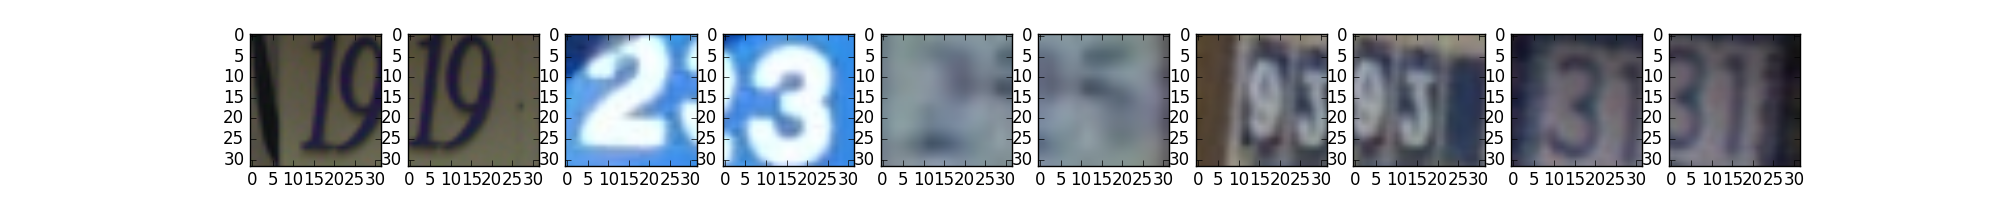
\includegraphics[width=80mm]{train_first10.png}}
	\caption{\label{Figure 1}
		First 10 images in the training set}
\end{figure}

\hrulefill

\section{Methods and Results}
\subsection{K-Nearest Neighbor}
\indent \indent We first used K-nearest neighbors (KNN) to learn over the training set and predict labels in the test set. Having performed 10-fold cross validation, we found that k = 15 gave the best validation accuracies, with average being 0.51 and relatively small standard deviation (Figure 2). With k = 15, the accuracy of our predictions came to be 0.49.

\begin{figure}[!tpb]
	\centerline{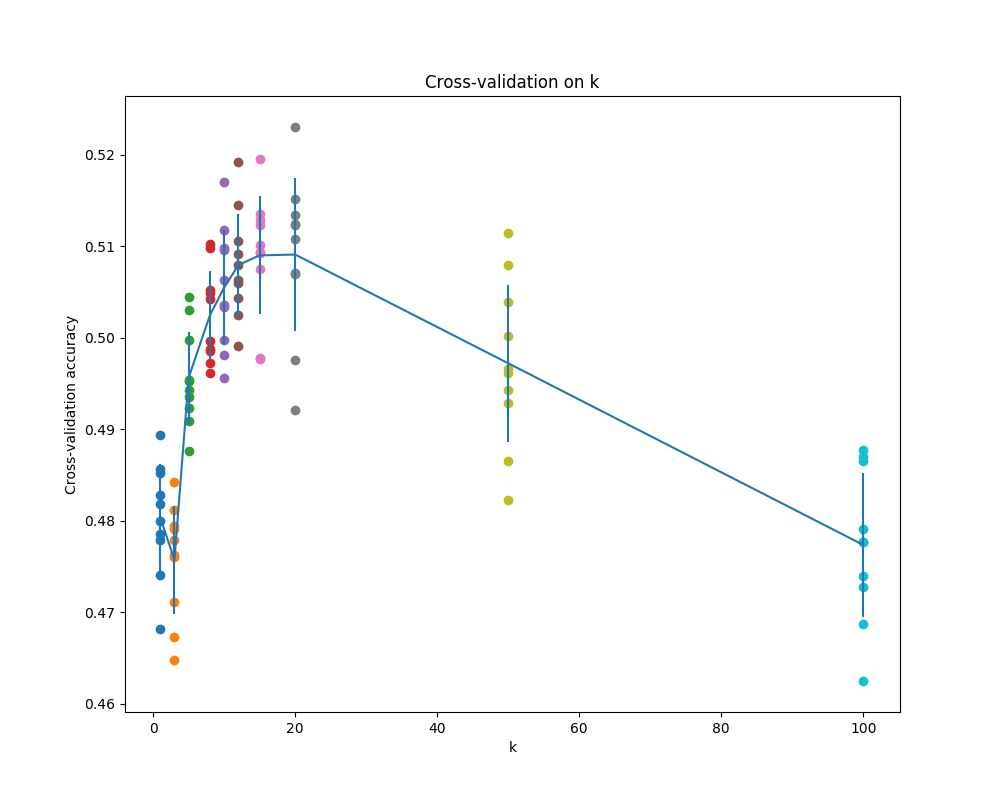
\includegraphics[width=80mm]{knn.png}}
	\caption{\label{Figure 2}
		10x cross validation shows that k = 15 is the best k for KNN classifier}
\end{figure}

\indent \indent In order to improve our accuracy, we tried a few image preprocessing methods. 
We converted RGB to grayscale using a weighting method, which takes into account human's different perception of different colors (new grayscale image = ( (0.3 * R) + (0.59 * G) + (0.11 * B)). This resulted in a slight increase in test accuracy (at k=15), from 0.49 to 0.52. Moreover, normalizing the grayscale inputs in order to remove trivial features led to further increase in test accuracy (=0.53).

\subsection{One vs All}
\indent \indent Next, we tried OVA with different regularization terms (lambda). (more on OVA, why we expect it to succeed)
Lambda = 0, 1, and 50 all yielded prediction accuracy of 0.24, which is much lower than that of KNN 

\subsection{Softmax}
\indent \indent Softmax is a multi-class logistic regressioin classifier. It outputs normalized probabilities assigned to each label by minimizing the cross-entropy between the estimated class probabilities and the true distribution. 

 \indent When implementing Softmax on SVHN data, hyperparameter search gave us best validation accuracy of 0.23 with learning rate = 1e-7 and regularization = 5e+5 without normalization. With normalization, we achieved a higher best validation accuracy of 0.26 with learning rate = 5e-7 and regularization = 1e+5. This is consistent with achieving a higher accuracy by normalizing the images in KNN. However, the test accuracy was only 0.1.



\subsection{Fully Connected Neural Network}
5 layer fully connected net w RGB:\\
batch size = [50, 100]\\
update rule = ['adam', 'sgd', 'rmsprop', 'sgd\_momentum']\\
lr = [1e-2, 1e-3, 1e-4]\\
weight scale = [1e-2, 5e-2, 1e-3, 1e-4]\\
\\
best parameters: batch size = 50; weight scale = 0.05; update rule = adam; lr = 0.001\\
\\
Test set accuracy: 0.73138\\
\\
Conversion from RGB to YUV\\
Validation set accuracy:  0.79436 @ 20 epochs à Test set accuracy: 0.77762\\



\subsection{Convolutional Neual Network}
\indent \indent Our next logical step was to try CNN as it is known to perform well when the inputs are images. Regular neural networks do not scale well to larger images as they tend to result in a huge number of parameters, which then also leads to overfitting. In CNN, neurons in a layer will only be connected to a small region of the layer before it, instead of being fully connected.  Moreover, CNNs constrain the architecture in a way more suitable for images as inputs. The layers of CNN have neurons arranged in three dimensions - width, height, and depth. We can manipute the final output layer to have dimensions 1x1x10 so that CNN architecture can reduce a full image into a single vector of scores for each classes. 

\indent Our CNN consists of two repeats of [Conv - ReLU - Pool] layers. Before being put through layers, the input images (32x32x3) are preprocessed by normalization and grayscale conversion, which flattens them to be (32x32x1). The first Conv layer has 32 filters with the size of 5x5 and stride = 1. Our second Conv layer has 64 filters with the size of 3x3 and stride = 1. Here, each image is zero padded automatically so that the output size will remain the same. ReLU layer applies an elementwise activation function of max(0,x). Pool layer carries out 2x2 max pooling. 

\indent After the two repeats of [Conv - ReLU - Pool] layers, we implement one fully-connected layer. In order to prevent overfitting, we include a dropout method, which randomly drops units and their connections during training. Moreover, we use Adaptive Moment Estimation (ADAM) as our gradient descent algorithm. Lastly, our readout layer uses softmax as a loss function. Using this three-layered CNN allowed us to reach 0.88 as validation accuracy and 0.86 as test accuracy. 

\section{Discussion}


\section {References}
\begin{description}
	\item[$\cdot$] http://cs231n.github.io/linear-classify/\#softmax
	\item[$\cdot$] https://msdn.microsoft.com/en-us/library/azure/dn905887.aspx?f=255\&MSPPError=-2147217396
	\item[$\cdot$] http://cs231n.github.io/convolutional-networks/
\end{description}

\end{document}